\documentclass[11pt]{article}
\usepackage[margin=1in]{geometry}
\usepackage{amsmath,amssymb}
\usepackage{graphicx}
\usepackage[colorlinks=true,linkcolor=blue,citecolor=blue,urlcolor=blue]{hyperref}
\newcommand{\Tr}{\operatorname{Tr}}

\title{Operational Influence Proxies in a TFIM Surrogate:\\
Non-Monotonicity and a Controlled $\omega = 0$ Witness Floor Mechanism\\
{\normalsize Version 2}}
\author{Lluis Eriksson\\ Independent Researcher\\ \texttt{lluiseriksson@gmail.com}}
\date{January 2026 (v1); July 2026 (v2)}

\begin{document}
\maketitle

\begin{abstract}
We study spatial influence detection in a transverse-field Ising chain
(TFIM) subjected to localized Markovian noise. Using an operational
one-site trace-distance influence proxy computed from TEBD combined with
Monte Carlo wavefunction (MCWF) sampling, we test whether remote
dissipation produces an identifiable nonzero asymptotic influence offset
(a ``floor'') as a function of separation $\epsilon$. Uncertainties are
estimated by trajectory bootstrap and model selection is performed between
exponential decay and exponential-plus-offset forms using both BIC and the
finite-sample corrected criterion AICc. In the TFIM surrogate regimes
explored, we find no robustly identifiable floor for both dephasing and
amplitude-damping channels; instead, the influence proxy is non-monotone
in separation, consistent with coherent finite-size structure superimposed
on average attenuation. To demonstrate that floors can exist as a
controlled mechanism independent of fragile spatial fits, we present a
Davies/witness stress test: for nonzero zero-frequency bath weight
$\gamma(0) > 0$, a commutator witness yields a strictly positive lower
bound on an effective decay envelope. Exact-diagonalization calculations
show this lower bound is robust to enlarging the observable support and to
variations in inverse temperature. \emph{v2 adds:} a synthetic-injection
power analysis showing that over the sampled one-octave window
$\epsilon \in [16, 32]$ with $n = 5$ points, a constant floor is nearly
degenerate with a slow exponential -- AICc essentially never detects a
floor and even BIC requires $D_0 \sim 30\sigma$ -- so ``no identifiable
floor'' is in part a design limitation, now stated as such; a fully
declared exact-diagonalization benchmark for the witness (v1 did not
record its ED parameters), regenerable from scratch by the shipped suite;
a null case showing the witness switches off ($\kappa_{\min} \sim
10^{-29}$) for couplings with vanishing $\omega = 0$ component;
an invariant-subspace caveat for the envelope interpretation; and series
cross-references.
\end{abstract}

\section{Introduction}
Locality constraints in quantum lattice systems limit how quickly and how
strongly perturbations influence distant degrees of freedom \cite{LR}.
Operational influence detection often relies on reduced-state or
local-observable proxies rather than direct access to a full many-body
channel. A recurring question is whether such proxies exhibit a nonzero
asymptotic offset (a ``floor'') in separation $\epsilon$, or whether they
decay without a detectable offset.

This paper has two goals. First, we evaluate a TFIM numerical surrogate
using a one-site trace-distance influence proxy under localized Markovian
noise, and we test for an identifiable floor using statistically
controlled model selection. Second, we provide a controlled stress test in
which a floor mechanism exists in a precise sense: as a witness-based
lower bound in a Davies-type $\omega = 0$ sector with $\gamma(0) > 0$
\cite{Davies, BP, Spohn}. The contrast clarifies a key message: the
existence and detectability of floors depends on both the chosen
operational proxy and on low-frequency bath structure.

\paragraph{Series context (added in v2).} This note is the numerical
companion of the $\omega = 0$-floor block of the coherence-maintenance
series: the windowed-proxy withdrawal and exact local-sink suppression of
2512.0064 v2 \cite{S0064} (the non-monotonicity found here is the same
phenomenon that motivated that withdrawal), the Davies-class
ceiling/floor envelopes of 2512.0070 v2 \cite{S0070}, and the entropic
interface 2601.0020 \cite{S0020}, whose Appendix~C reproduces
Figures~\ref{fig:tail} and \ref{fig:witness} below as illustrations. The
proxy-discipline lesson (power analysis before interpreting nulls) follows
2512.0105-style methodology \cite{S0105}.

\section{TFIM surrogate: model, proxy, and inference pipeline}
\subsection{Hamiltonian}
We consider a TFIM chain of length $N$ with open boundary conditions and
Hamiltonian
\[
H = -J\sum_{i=1}^{N-1} X_i X_{i+1} - h\sum_{i=1}^{N} Z_i .
\]
(Equivalent to the ZZ--X convention by a global basis rotation.)

\subsection{Noise channels and geometry}
We study localized Markovian noise applied on a set of sites separated
from a probe site $S$ by a distance $\epsilon$: dephasing (jump operators
$\propto Z$) and amplitude damping (jump operators $\propto \sigma^- =
(X - iY)/2$). For each separation $\epsilon$, noise acts on a small region
$\mathcal{N}(\epsilon)$ at distance $\epsilon$ from $S$.

\subsection{Operational influence proxy}
For each $\epsilon$, we compare (i) a noisy evolution with dissipation at
$\mathcal{N}(\epsilon)$ to (ii) a clean unitary evolution under $H$. With
$\bar\rho^{\rm noisy}_S(t)$ the trajectory-averaged reduced state at the
probe and $\rho^{\rm uni}_S(t)$ the unitary reference (independent of
$\epsilon$), define the instantaneous trace-distance influence
$D_{\rm tr}(t;\epsilon) := \tfrac12 \| \bar\rho^{\rm noisy}_S(t) -
\rho^{\rm uni}_S(t) \|_1$ and windowed aggregates
$D^{\mathcal{A}}_{\rm tr}(\epsilon)$, $\mathcal{A} \in \{\max, {\rm mean},
{\rm rms}\}$, over post--light-cone windows $t_0(\epsilon) =
\alpha\epsilon/v$, $t_1 = t_0 + \tau$.

\subsection{Uncertainty estimation and model selection}
Uncertainties are bootstrap 16--84\% intervals over trajectories. We
compare $M_{\rm exp}: D(\epsilon) = Ae^{-a\epsilon}$ and
$M_{\rm floor}: D(\epsilon) = D_0 + Ae^{-a\epsilon}$ ($A, D_0 \ge 0$) by
weighted least squares with a log-spaced grid over $a$, summarized by
$\Delta{\rm BIC}$ and $\Delta{\rm AICc}$ with ${\rm BIC} = \chi^2 +
k\log n$, ${\rm AICc} = \chi^2 + 2k + 2k(k+1)/(n-k-1)$ \cite{BA, HT}. For
the tail-only fits below ($n = 5$), the AICc correction contributes
$\approx 18$ additional units to the offset model ($k = 3$ vs $k = 2$), so
$\Delta{\rm AICc} \approx 20$ indicates insufficient support for an extra
parameter at small $n$, not strong physical evidence against $D_0$.

\subsection{Power of the no-floor conclusion (added in v2)}
\label{sec:power}
A null is informative only relative to what the design could detect. The
suite (Section~\ref{sec:verif}) injects known floors $D_0$ into synthetic
data with the sampled design ($n = 5$, $\epsilon \in \{16, 20, 24, 28,
32\}$, matched noise) and runs the identical pipeline. Result: AICc
essentially never selects the floor model (it requires
$\Delta\chi^2 > 20$), and even BIC reaches 80\% detection only near
$D_0 \sim 30\sigma$. The mechanism is a \emph{design degeneracy}: over a
one-octave window, a slow exponential ($a \to 0$) mimics a constant
offset, so the criteria cannot separate them regardless of sample size.
Consequently, the correct reading of Section~\ref{sec:results} is: no
floor is identifiable \emph{and} the design could not have identified any
floor smaller than the in-window signal itself; identifying subdominant
floors requires a wider $\epsilon$ aspect ratio, amplitude constraints,
or channel-specific nulls. This sharpens, rather than weakens, the
contrast with the certified witness mechanism of
Section~\ref{sec:witness}.

\section{TFIM surrogate results}
\label{sec:results}
\subsection{Dephasing deep tail ($N = 80$, post--LC)}
For dephasing at $N = 80$, $\epsilon \in \{16, 20, 24, 28, 32\}$:
$D^{\mathcal{A}}_{\rm tr}(\epsilon)$ is non-monotone (a bump appears),
indicating coherent finite-size structure superimposed on average
attenuation. Model selection yields no supported/identifiable floor for
all aggregators: $\Delta{\rm BIC} \approx 1.5$--$1.6$,
$\Delta{\rm AICc} \approx 20$ -- i.e.\ $\chi^2$ improvement $\approx 0$
(pure penalty), consistent with no floor signal \emph{within the power
limits of Section~\ref{sec:power}}.

\subsection{Amplitude damping corroboration ($N = 24$)}
At $N = 24$, $\epsilon \in \{2, 4, 6, 8, 10\}$: non-monotone dependence,
no-floor model favored across aggregators ($\Delta{\rm BIC} \approx 1.6$,
$\Delta{\rm AICc} \approx 20$), same power caveat.

\begin{figure}[h]\centering
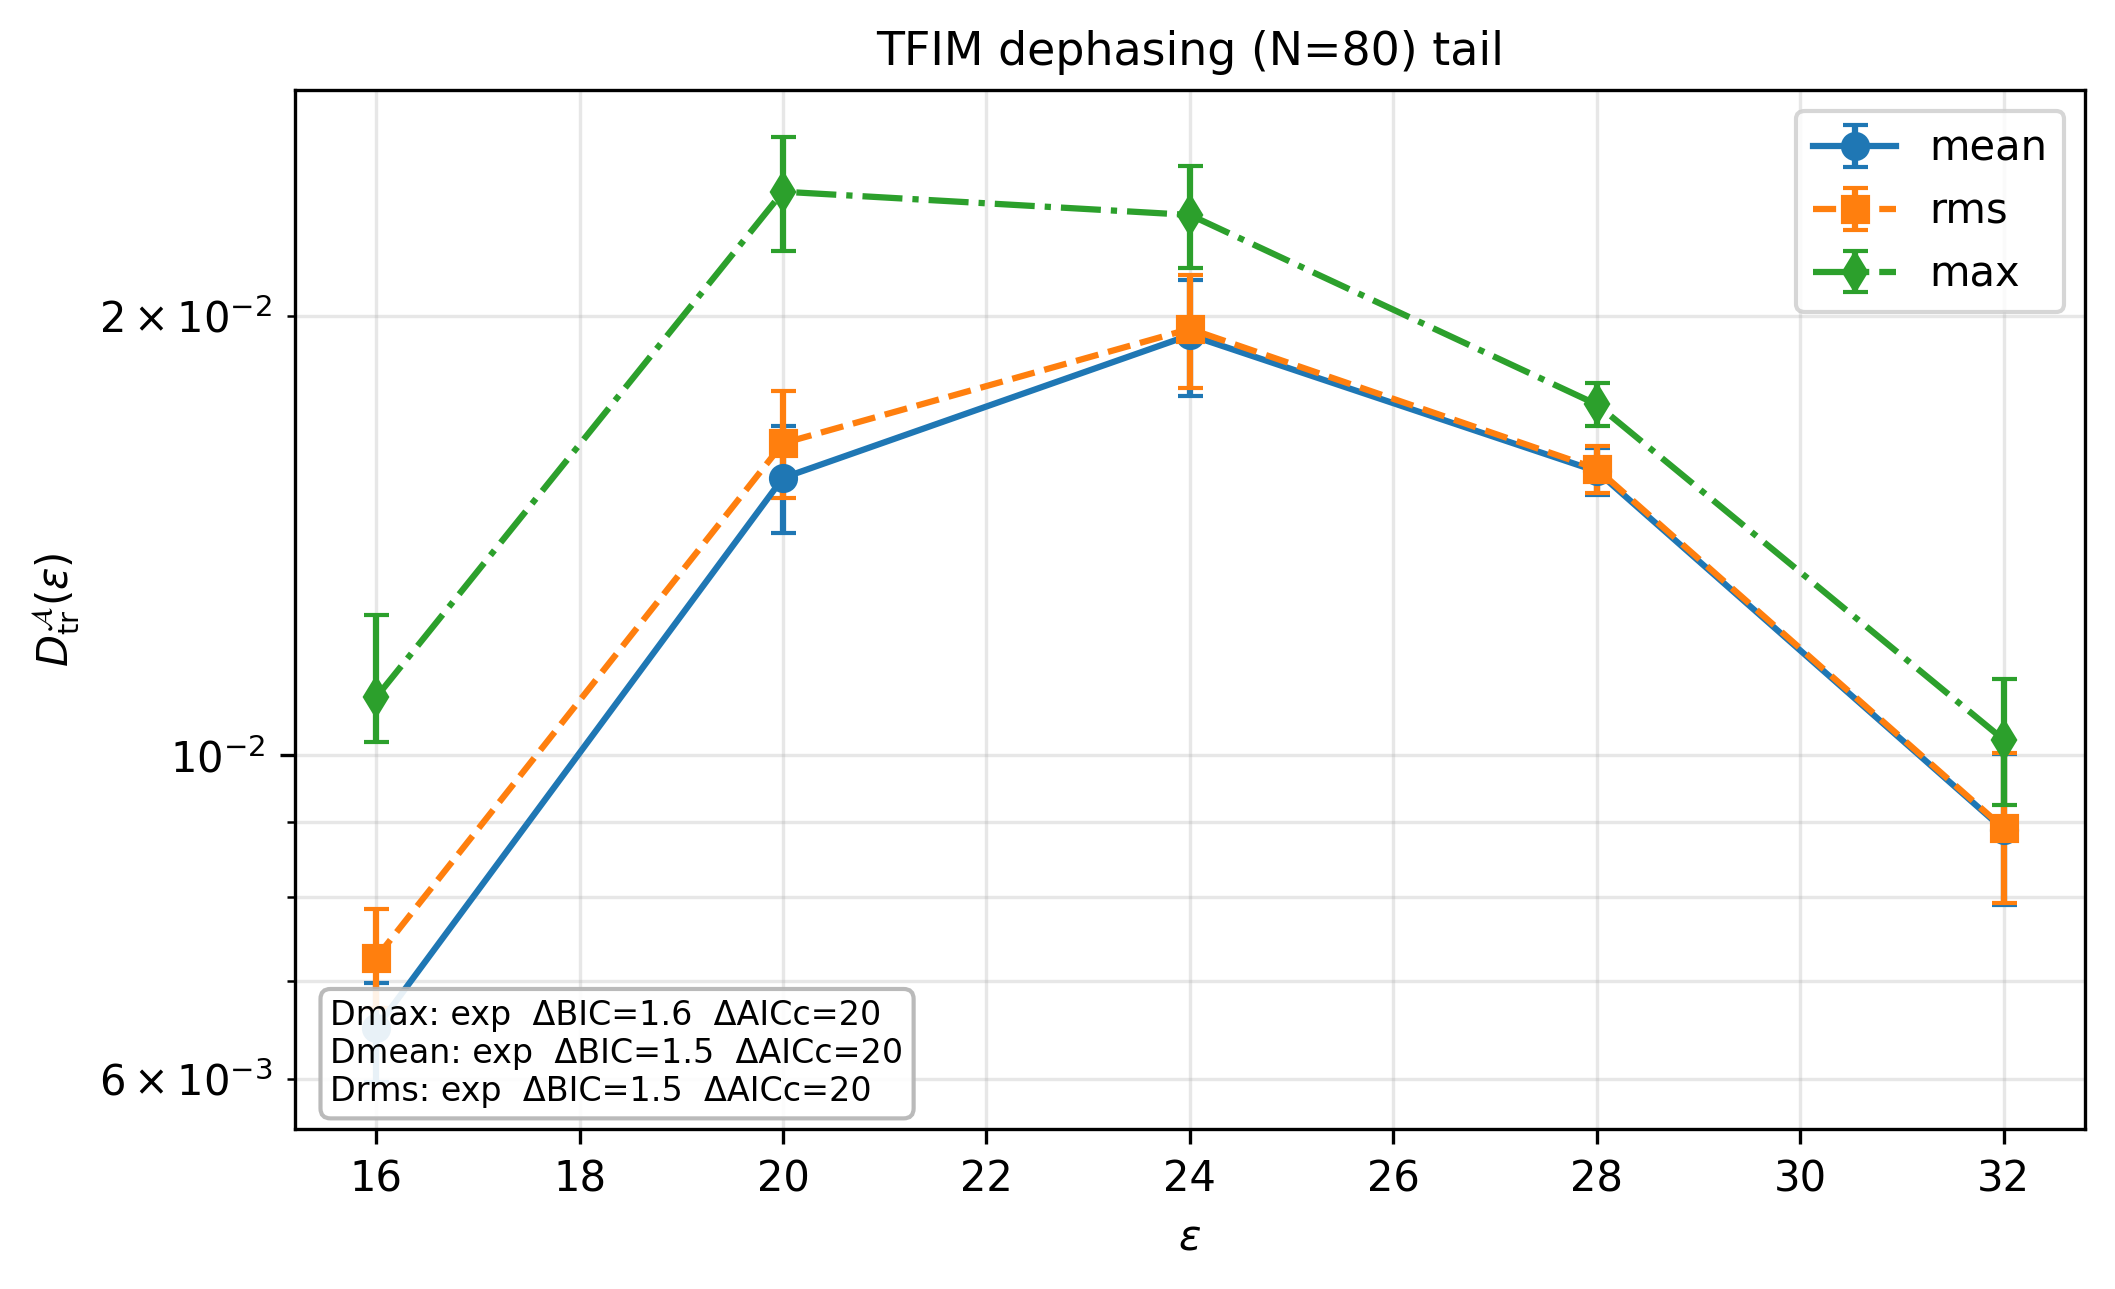
\includegraphics[width=0.8\textwidth]{fig1_dephasing_tail.png}
\caption{TFIM dephasing tail ($N = 80$): windowed influence proxy with
bootstrap 16--84\% intervals. Model selection supports the no-floor model
for $\mathcal{A} \in \{\max, {\rm mean}, {\rm rms}\}$; see
Section~\ref{sec:power} for what this does and does not imply.}
\label{fig:tail}
\end{figure}
\begin{figure}[h]\centering
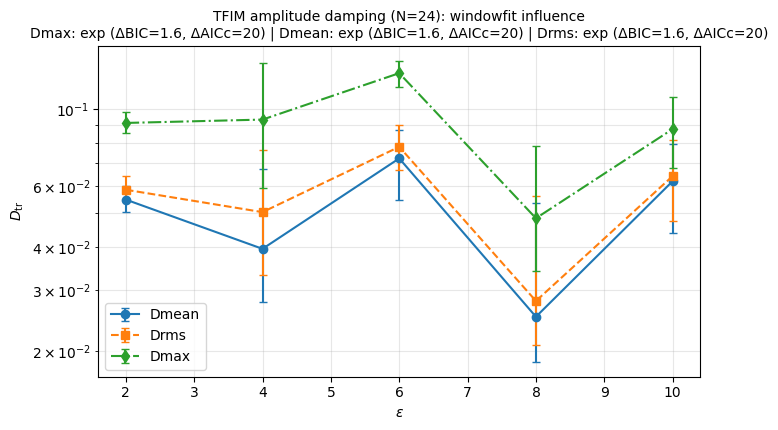
\includegraphics[width=0.62\textwidth]{fig2_ampdamp.png}
\caption{Influence proxy under amplitude damping ($N = 24$); error bars
are bootstrap 16--84\% intervals. Non-monotone in $\epsilon$.}
\end{figure}
\begin{figure}[h]\centering
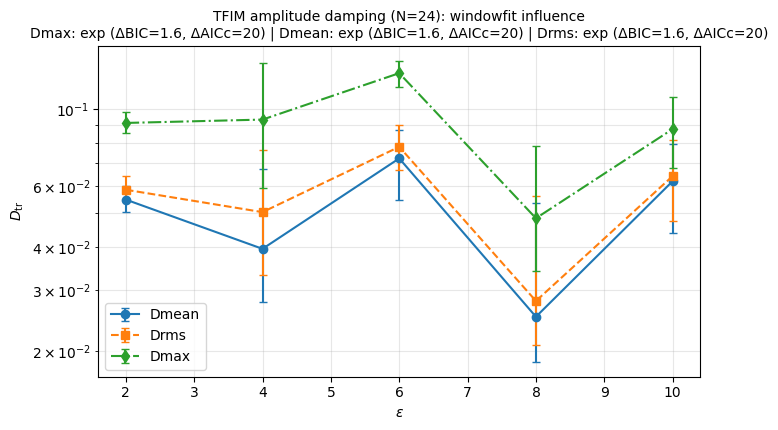
\includegraphics[width=0.62\textwidth]{fig3_ampdamp_summary.png}
\caption{Processed influence summary for the amplitude-damping check
($N = 24$).}
\end{figure}

\paragraph{Data availability (added in v2).} Trajectory-level TEBD/MCWF
data are not shipped with this version; the figures are unchanged from
v1. The witness computations of Section~\ref{sec:witness}, by contrast,
are fully regenerable from scratch by the verification suite.

\section{Davies/witness stress test: controlled $\omega = 0$ floor
mechanism}
\label{sec:witness}
\subsection{Scope}
We use a controlled $\omega = 0$-channel witness (Dirichlet-form
identity) as a stress test; we do not reconstruct the full Davies
generator. This is a certified lower-bound mechanism statement, not a
claim about the full $\epsilon$-dependence of physical decoherence rates
in the TFIM surrogate. \emph{(Added in v2)} Moreover, as an instantaneous
Dirichlet-ratio bound it controls decay of observables in the witness
sector only under the usual invariant-subspace extension (cf.\ the
Gr\"onwall step in 2601.0020 \cite{S0020}); we use the term
``envelope'' in that conditional sense.

\subsection{Definitions: $S(0)$ and $\mathcal{A}_\epsilon$}
With $\{\Pi_n\}$ the spectral projectors of $H$, define $S(0) := \sum_n
\Pi_n S \Pi_n$ (energy-block-diagonal part of the system--bath coupling
$S$); $S(0)$ is generally nonlocal in real space. $\mathcal{A}_\epsilon$
is the span of traceless Pauli strings on a block of length $L$ starting
at site $k = j_0 + \epsilon$ (open chain), $j_0 = \lfloor N/2 \rfloor$.

\subsection{Witness lower bound}
With $\sigma$ a reference Gibbs/KMS state and $\langle A, B
\rangle_\sigma := \Tr(\sigma^{1/2} A^\dagger \sigma^{1/2} B)$,
\[
\kappa(\epsilon) \ge \kappa_{\min}(\epsilon) := \frac{\gamma(0)}{2}\,
R_{\rm opt}(\epsilon),
\qquad
R_{\rm opt}(\epsilon) := \max_{O \in \mathcal{A}_\epsilon}
\frac{\|[S(0), O]\|^2_{2,\sigma}}{\|O\|^2_{2,\sigma}} ,
\]
so any $R_{\rm opt}(\epsilon) > 0$ certifies $\kappa_{\min}(\epsilon) > 0$
whenever $\gamma(0) > 0$.

\subsection{Exact diagonalization: declared benchmark (revised in v2)}
\label{sec:edbench}
v1 reported ED ranges at $N = 10$ without recording the parameters
$(J, h, S)$, which made exact reproduction impossible. v2 fixes a fully
declared benchmark, regenerated from scratch by the suite: $N = 10$,
$J = 1$, $h = 1.05$, $S = Z$ at the center site, $\gamma(0) = 0.1$,
$\epsilon \in \{1, 2, 3\}$, $\beta \in \{0.5, 1, 2\}$, blocks $L \in
\{1, 2\}$. The witness-based lower bound ranges
\[
\kappa_{\min} \in [1.79 \times 10^{-3},\, 5.72 \times 10^{-3}]
\ (L = 1),
\qquad
\kappa_{\min} \in [4.31 \times 10^{-3},\, 6.82 \times 10^{-3}]
\ (L = 2):
\]
strictly positive throughout, increasing with observable support, robust
in $\beta$ -- the same qualitative structure as v1's figures (v1's
magnitudes are same-order; its exact parameters were not preserved).
\emph{Null case (added in v2):} for $S = X$ at the center site the
$\omega = 0$ component essentially vanishes and the suite finds
$\kappa_{\min} \sim 10^{-29}$: the floor mechanism switches off for
couplings with no zero-frequency diagonal part, sharpening the message
that low-frequency bath structure -- not locality alone -- controls
floor existence.

\begin{figure}[h]\centering
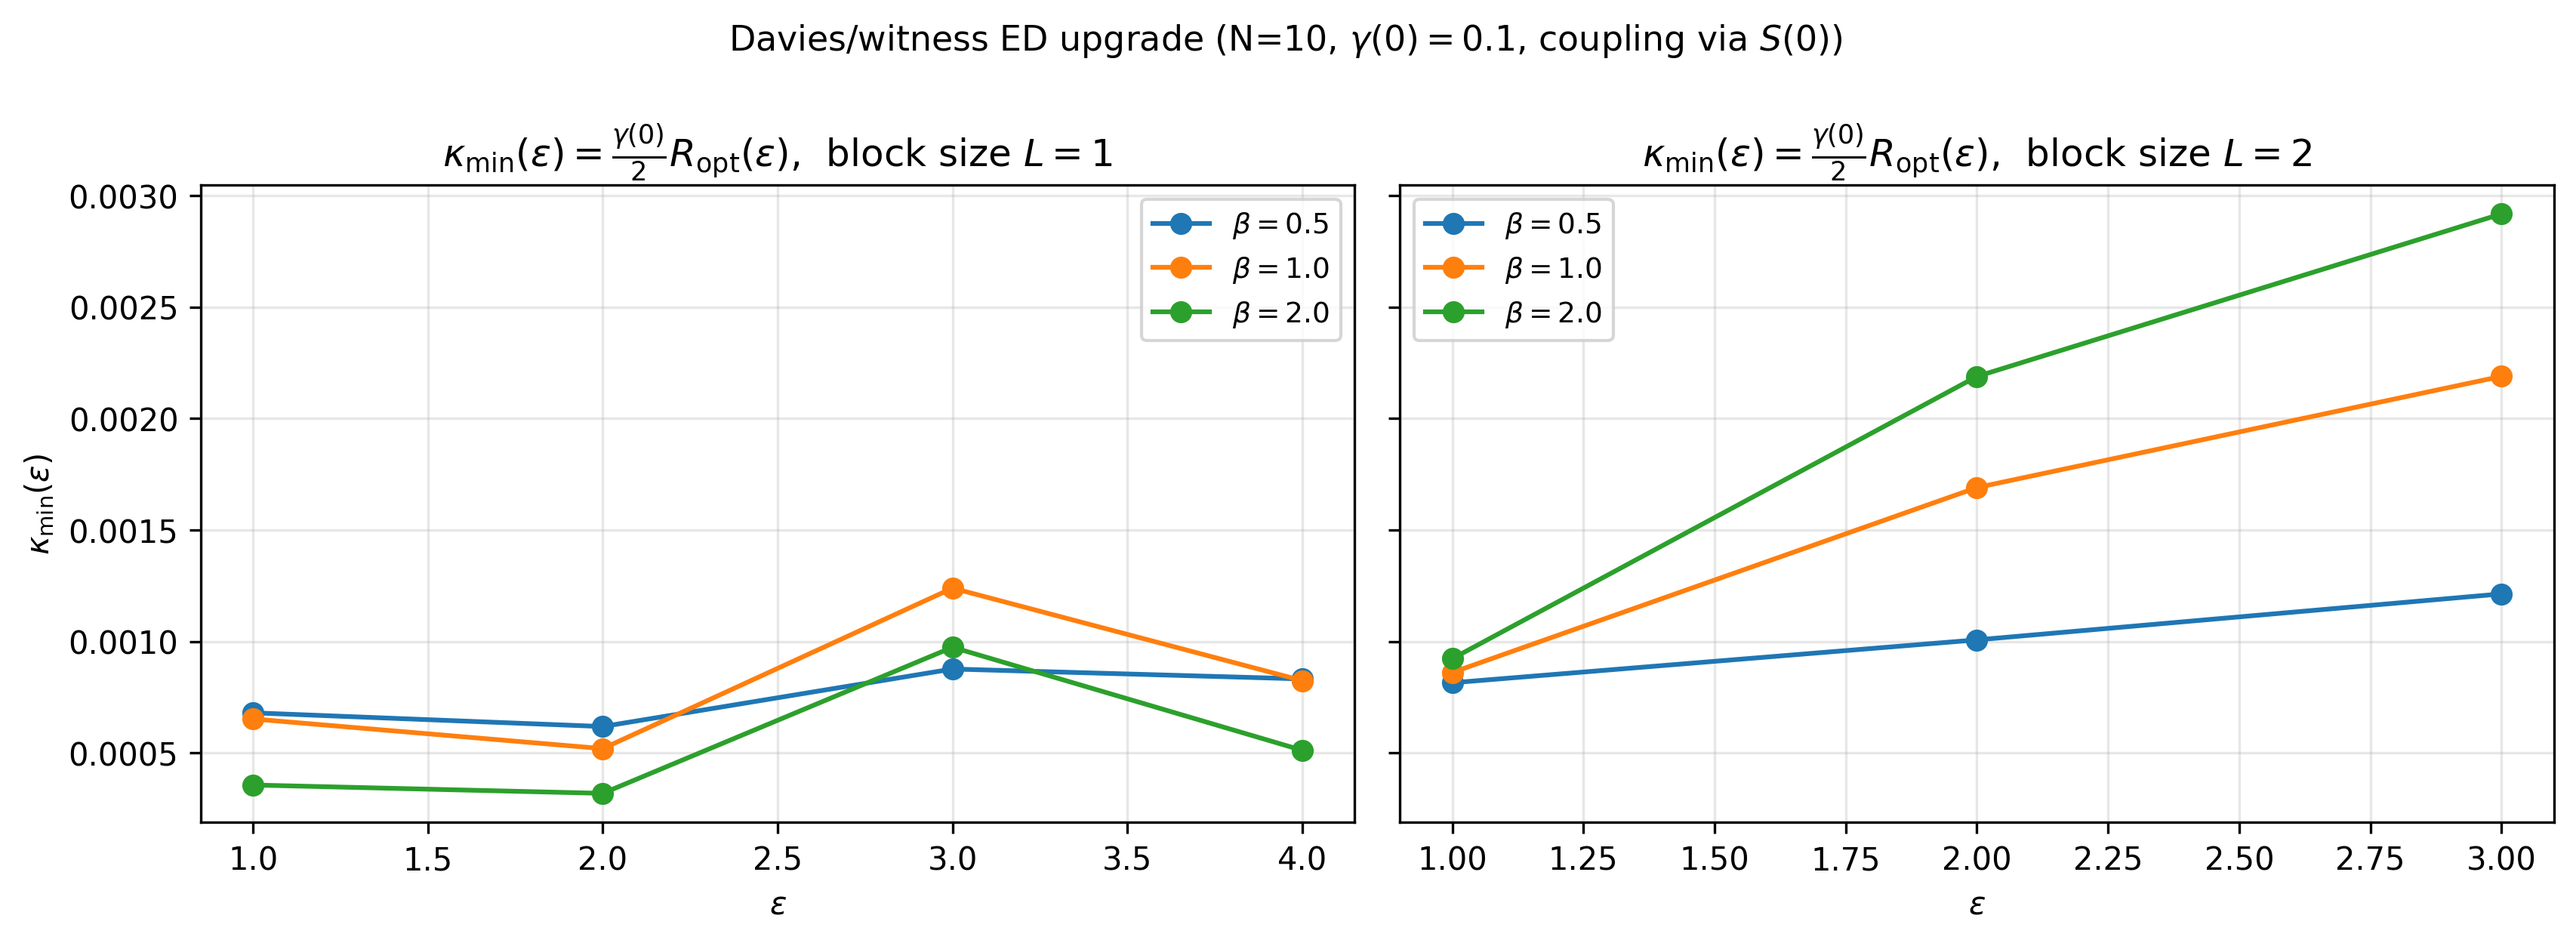
\includegraphics[width=0.85\textwidth]{fig4_witness_ed.png}
\caption{Davies/witness ED ($N = 10$, v1 figure): witness lower bound
$\kappa_{\min}(\epsilon) = \tfrac{\gamma(0)}{2} R_{\rm opt}(\epsilon)$,
$\gamma(0) = 0.1$, for $L = 1, 2$ and $\beta \in \{0.5, 1, 2\}$. See
Section~\ref{sec:edbench} for the v2 declared benchmark.}
\label{fig:witness}
\end{figure}

\section{Verification suite (added in v2)}
\label{sec:verif}
\texttt{verification/2601-0022/verify\_2601\_0022.py} (pure NumPy/SciPy,
$\sim$70 s): Part A regenerates the declared witness benchmark of
Section~\ref{sec:edbench} from scratch (ED, KMS inner products,
generalized eigenproblem over Pauli blocks) together with the $S = X$
null case; Part B runs the synthetic floor-injection power analysis of
Section~\ref{sec:power} (60 repetitions per injected level, identical
fitting pipeline). Reference output ships alongside.

\section{Discussion and conclusions}
The TFIM surrogate results show that, for this operational one-site
trace-distance proxy in the explored regimes, an offset parameter $D_0$
is not supported/identifiable under either dephasing or amplitude
damping -- with the v2 power analysis quantifying exactly how strong a
floor would have had to be for the design to see it, and identifying the
slow-exponential/floor degeneracy of narrow $\epsilon$ windows as the
limiting factor. The observed non-monotonicity in $\epsilon$ indicates
coherent finite-size structure that limits the interpretability of
strictly monotone envelope fits -- the same phenomenon behind the
windowed-proxy withdrawal of 2512.0064 v2 \cite{S0064}. In contrast, the
Davies/witness stress test demonstrates an explicit, certified and now
exactly reproducible floor mechanism when $\gamma(0) > 0$, which switches
off when the coupling lacks a zero-frequency component. Floors are not
universal across operational proxies; low-frequency bath structure and
the observable family determine whether a floor exists, and the sampling
design determines whether it could even be detected.

\section*{Note added in v2}
No v1 result is retracted: the no-floor model selection, the
non-monotonicity, and the positive witness mechanism all stand. v2 adds
what a careful referee would demand: (1) the power analysis of
Section~\ref{sec:power} (the no-floor null is design-limited: AICc
cannot detect floors at $n = 5$; BIC needs $D_0 \sim 30\sigma$ due to the
slow-exponential degeneracy); (2) a fully declared, from-scratch
reproducible ED benchmark for the witness (v1's ED parameters were not
recorded), with same-order agreement and identical qualitative structure;
(3) the $S = X$ null case ($\kappa_{\min} \sim 10^{-29}$); (4) the
invariant-subspace caveat on ``envelope''; (5) series cross-references
and the data-availability statement; (6) Figure~3 caption cleaned.

\begin{thebibliography}{12}
\bibitem{LR} E.~H. Lieb and D.~W. Robinson, Commun. Math. Phys.
\textbf{28} (1972) 251--257.
\bibitem{Davies} E.~B. Davies, Commun. Math. Phys. \textbf{39} (1974)
91--110.
\bibitem{BP} H.-P. Breuer and F. Petruccione, \emph{The Theory of Open
Quantum Systems}, Oxford University Press (2002).
\bibitem{Spohn} H. Spohn, J. Math. Phys. \textbf{19} (1978) 1227--1230.
\bibitem{BA} K.~P. Burnham and D.~R. Anderson, \emph{Model Selection and
Multimodel Inference}, 2nd ed., Springer (2002).
\bibitem{HT} C.~M. Hurvich and C.-L. Tsai, Biometrika \textbf{76} (1989)
297--307.
\bibitem{S0064} L. Eriksson, ai.viXra:2512.0064 (2025; v2 2026).
\bibitem{S0070} L. Eriksson, ai.viXra:2512.0070 (2025; v2 2026).
\bibitem{S0020} L. Eriksson, ai.viXra:2601.0020 (2026; v2 2026).
\bibitem{S0105} L. Eriksson, ai.viXra:2512.0105 (2025; v2 2026).
\end{thebibliography}
\end{document}
